\chapter{Implementation structure}
Implementation chapter reveals the overall application architecture overview. Its purpose is to provide the information using which the experienced developer can understand and further improve the project. 

At first, we summarize the overall project architecture and the services involved in our solution. Then we explain the base parts of our application and how the application uses them. In the end, we focus on the implementation details of some of the application parts and explain the things that are not obvious from the project structure and conventions.


\section{Project architecture}

The whole project consists of multiple services. Back-end application, Errbit for error monitoring, Kibana for accessing the logs from all of the running services and the front-end applications. Each of the services has its own domain. They all are behind the ngnix reverse proxy which analyses incoming HTTP requests and delivers them to the desired service \ref{services-scheme}.  
\begin{figure}[h]\centering
	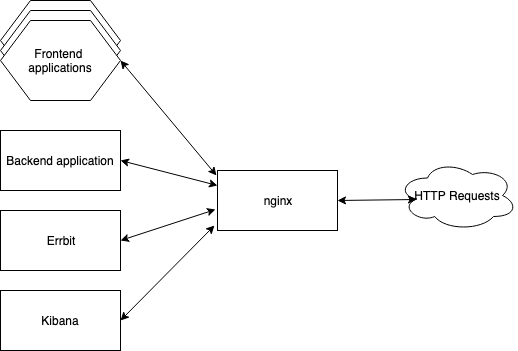
\includegraphics[scale=0.7]{architecture/services_architecture.png}
	\caption{Services scheme} 
	\label{services-scheme}
\end{figure} 

In the following scheme 
\ref{application-sw-stack-scheme} we can see the whole application software stack described in the technical analysis. We also display the external services and APIs that our application uses. We depict the communication channels between all the parts involved.
 \begin{figure}[h]\centering
 	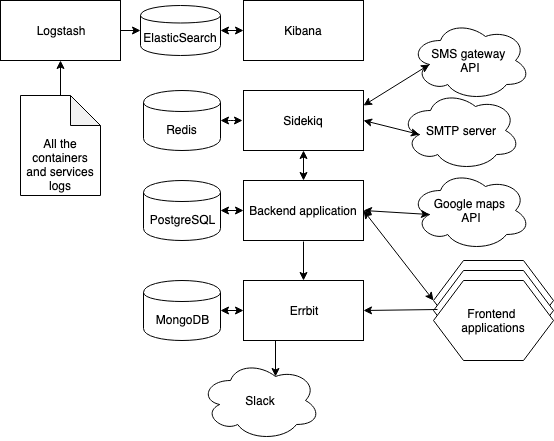
\includegraphics[scale=0.7]{architecture/services_technologies_scheme.png}
 	\caption{Application software stack scheme} 
 	\label{application-sw-stack-scheme}
 \end{figure} 
 



\section {Application architecture}

	In this section we describe all the key principles Ruby on Rails defines and how we work with them in our application. We describe important things the developer needs to know for further application development. 

	Ruby on Rails is MVC framework. We suppose the reader is familiar with the MVC\footnote{\url{https://en.wikipedia.org/wiki/Model\%E2\%80\%93view\%E2\%80\%93controller}} pattern.
	
	Ruby on Rails framework is tightly connected with the \textit{Convention over configuration} software design paradigm. In short it means that we as a programmer are forced to use Rails conventions otherwise the application will not run. During the application development we have to have in mind that the file and class names or the folder structure is directly connected with the whole application architecture.
	
	\subsection{Gemfile}
		Gemfile specifies library (gem) project dependencies. Each gem record also contains version specification based on which the libraries can be automatically updated. This file is similar to the \textit{package.json} file in javascript NPM projects.
	
	
	\subsection{Controllers}
		 All controllers in Ruby on Rails inherits from the \textit{ApplicationController}. Because we are writing REST API which may define next versions in the future, we decided to add one more layer - \textit{ApiV2Controller}. This controller base takes care about the API-specific general tasks such as authorization. All the controllers in our application are inherited from this \textit{ApiV2Controller} controller.
		
		Each public method (action) in the controller class usually corresponds to one API endpoint. For each resource we typically use this set of actions:
		\begin{itemize}
			\item index = display all entities
			\item show = show specific entity
			\item create
			\item update
			\item destroy		
		\end{itemize} 
	
	Each controller class is a in a separate file inside the \path{app/controllers} folder so you can get  the overview  of controllers used there.
	\subsection{Models}
		Ruby on Rails provide rich ORM library called \textit{ActiveRecord}, which is the implementation of the \textit{ActiveRecord design pattern}\footnote{\url{https://en.wikipedia.org/wiki/Active\_record\_pattern}}. We use this library for the whole communication with the database.
		
		In our application all of the models derive from the Rails \textit{ApplicationRecord} class. Each model class corresponds one database table. In model classes we also define attribute validations and relations with other models. We can find all the application models inside the \path{app/models} folder.
		
		\subsubsection{Concerns}
			Concerns contain separated logic used across more models. Concern is a Ruby module which is extending the Rails \textit{ActiveSupport::Concern} module. This module is then included in the desired models. 
			In our application we use the concerns for authentication, user roles and notifications - all of them are used by the Customer and Employee model, thus it is convenient to have them at a separate place. Concerns are located in the \path{app/models/concerns} folder.
		\subsubsection{Scopes}
			Another interesting pattern we use a lot in our application are model scopes. Scopes allows us to have defined commonly used filters or queries directly on the model class. For example we have scope \textit{dispatchers} for the \textit{Employee} model, which selects from the set of employees only dispatchers.
		
	\subsection{Validators}
		During the order model creation we ended up with the complicated validator definition. For the better code readability we decided to separate that validator to its own class. This class lies in the \path{app/validators} folder as recommended by Rails.
		
		Even though the orders validator is the only one such complicated that we felt the urge to separate it to its own file, this folder can be used in the future for other complicated validators in the application.
	
	\subsection{Database}
		The whole database layer is wrapped by the Ruby on Rails framework which provide us the tools to manage it.
		
		\subsubsection{Schema}
			Rails contains whole database schema with the table columns properties and table indexes in a text file \path{db/schema.rb}. The database schema of our application is displayed at \ref{database-schema} 	
			\begin{figure}[h]\centering
				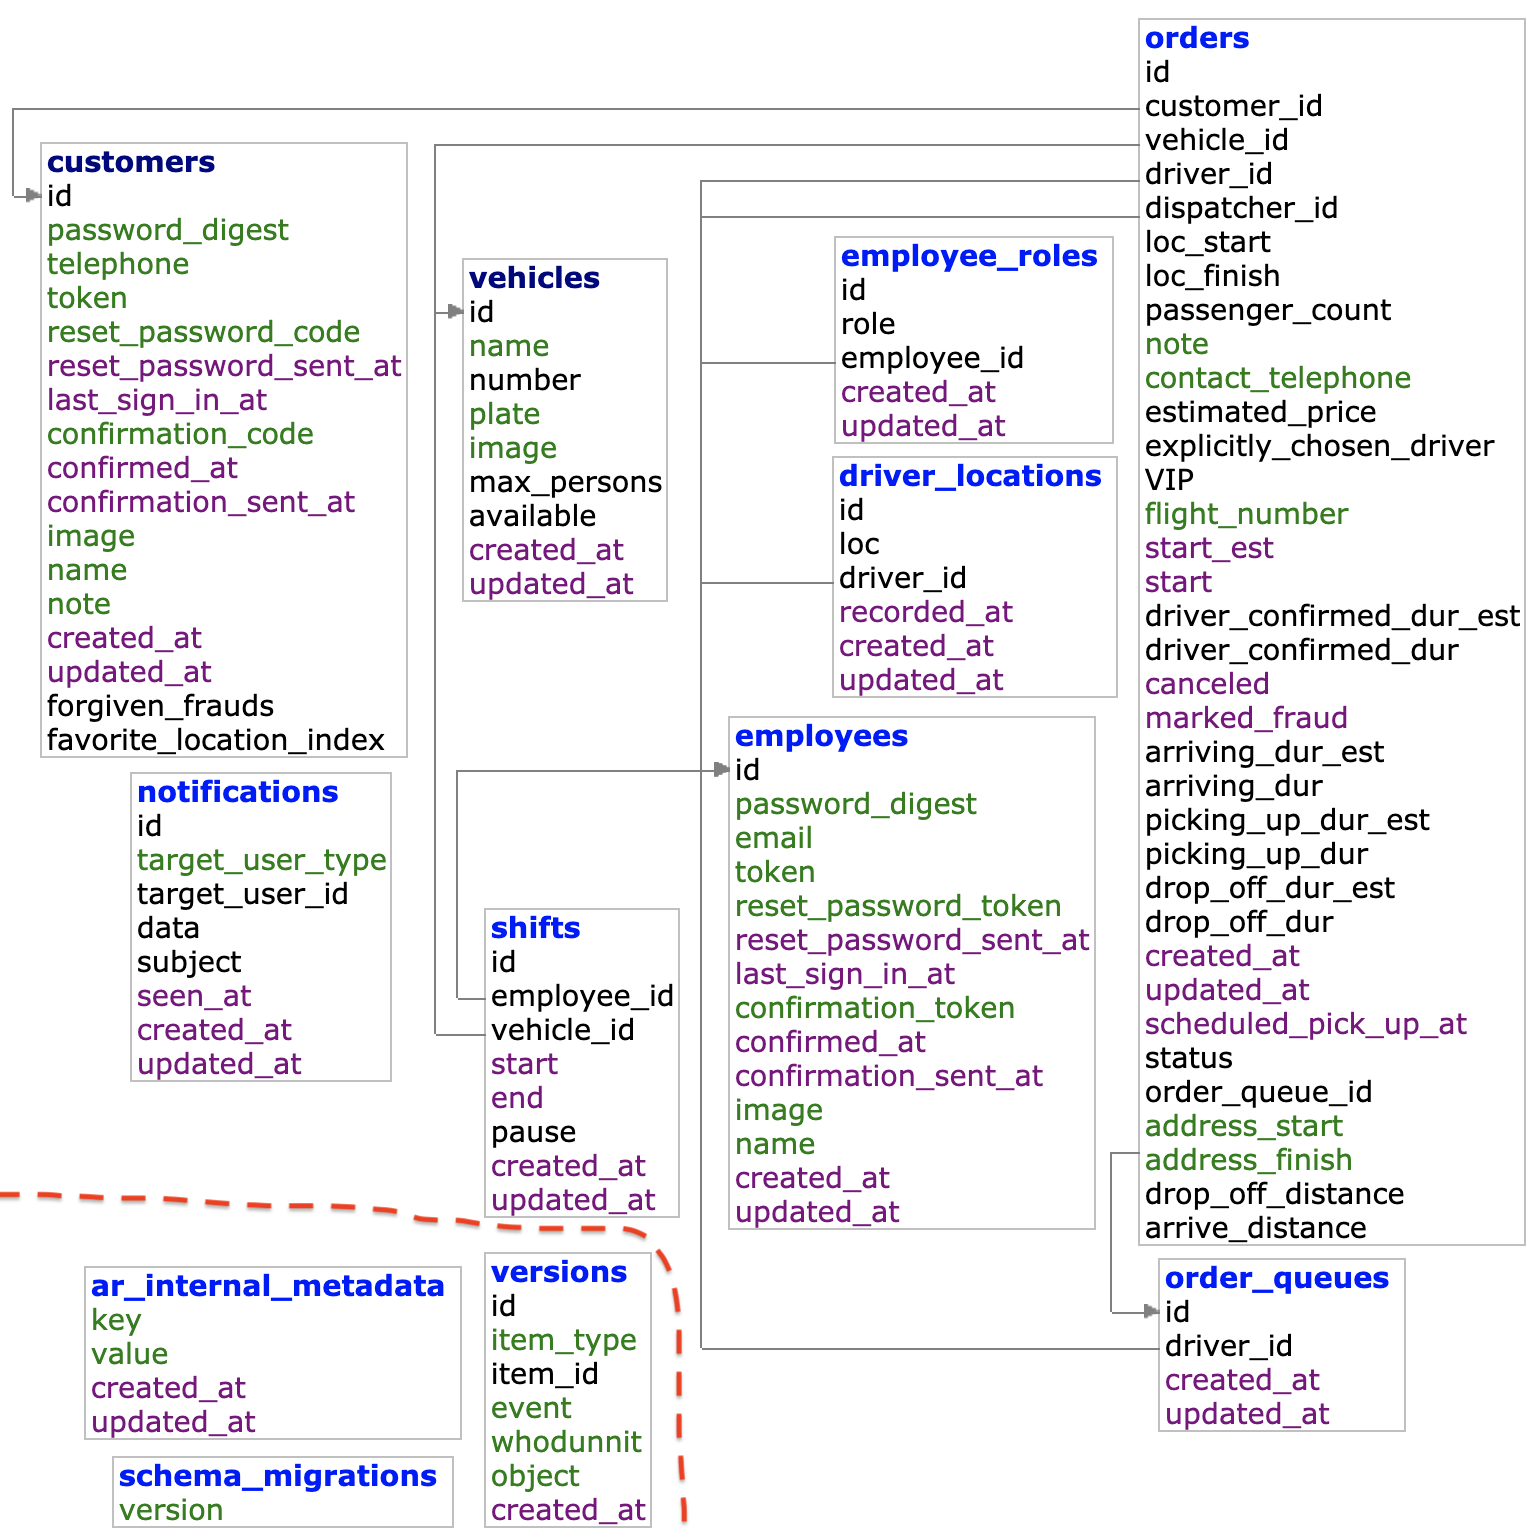
\includegraphics[scale=0.53]{db_schema.png}
				\caption{Database schema} 
				\label{database-schema}
			\end{figure} 
		
		\subsubsection{Migrations}
			All the tables in database are created and modified through the migrations. Migration is a class inherited from the Rails \textit{ActiveRecord::Migration} base class. It specifies how is the database transformed from the original state to a desired new one. These migrations are then executed during the database setup and allow us to modify the database in the future easily.
			
		All the migrations can be found inside the \path{db/migrate} folder.
		\subsubsection{Seeds}
			Seeds are a useful way to define the initial data. The data are inserted to the database when the \textit{rake db:seed} command is called. In our application we use it for setting up the initial administrator account.
			
			Seed script is located inside the \path{db/seeds.rb} file.
	
	\subsection{Workers}
		In general we can say that if there is a code in our application running asynchronously it is handled by workers. Each worker defines the asynchronous job. 
		
		Worker is a class which includes the \textit{Sidekiq::Worker} module and has public method perform that is called when the job is started. 
		
		The jobs are executed in parallel so we must have the code prepared for concurrency. Each job is automatically executed again in case of error. This implies that our jobs must be designed to run repeatedly with keeping the data consistent.
		
		In our application we use the workers for sending the SMS and emails. Besides that we use them for the favourite location indexing and the critical time order callback because the Sidekiq supports executing the jobs at specified time.

	\subsection{Helpers}
		 Helpers are meant for separating specific functions which are more general for the application and we want to have them separated for better code readability. Each helper is Ruby module containing the functions. We can find helpers in the \path{app/helpers} folder.
		
		In our application were helpers the first choice where to put the calculation of the distance between two coordinates. We use it in both controllers and workers and it is quite complex function to have it directly in place.
		
	\subsection{Mailers}
		Ruby on Rails has built-in support for sending emails. For each entity we derive class from the Rails \textit{ApplicationMailer} class. Each public method (action) in this class stands for one type of email. The Rails mailer provides us with out-of-the box asynchronous queue sending via SMTP - configured in \path{config/initializers} folder.
		 
		 The mail template which will be used for the email is specified in the \path{views/mailer_entity/mail_action.*}.
		 
		 In our application we use the mailers for sending the employees registration confirmations and forgotten password mails.

		
	\subsection{Policies}
		Policy classes hold the permission definitions which uses the Pundit gem. Basic principles how the policy definitions work and how they are connected with the rest of the application is described later in the \ref{implementation_authorization} 
	\subsection{Views}
		In the view part we have the JBuilder templates for the REST API endpoints. Besides that the view part contains email templates.
		
		Ruby on Rails takes care of connecting the controllers and mailers with the views. It works because we use Rails defined folder structure and file naming. For better understanding of our view architecture we are going to describe it.
		
		Each controller/mailer has folder with the same name inside the \path{app/views} folder. The folder path corresponds to the class inheritance path. For each controller/mailer action that uses the view part there exists a file with a same name as the action name.
		
		To avoid code duplication in templates we use partials. Partials are separated parts of views which can be imported in any of the view file. Partials are defined as files that start with underscore. 

		

		
		
	\subsection{Configurations}
		Ruby on Rails specifies that inside the  \path{config} folder lies all the application configurations. We describe the important ones which can be useful for future application modifications.
		\subsubsection{Initializers}
			Initializers handle the initialization and configuration of the modules and classes used across the application. Rails execute all the code in the \path{config/initializers} folder during the application start.
			
			The important initializers in our application there are initializers for Google Maps API, Sidekiq (asynchronous jobs), Kaminari (pagination), Lograge (logs formatting), CML (our order scheduler) and CORS.
			
		\subsubsection{Environments}
			General configurations which differs for the development, testing and production environment. Specifically we can find there mail and logs configurations. 
		\subsubsection{Database}
			Database YAML file defines which database we use on which environment. It specifies database server, credentials and the used database name.
		\subsubsection{Routes}
			Inside \path{config/routes.rb} file we define all the REST API endpoints. Ruby on Rails assumes that for each resource there exists controller with the same name. Each resource has set of default endpoints - \textit{index}, \textit{show}, \textit{create}, \textit{update} and \textit{destroy} action. 
			
			When the application receives a request, based on this configuration file Ruby on Rails decides, which controller it handles and calls the according action method on it.
		\subsubsection{Sidekiq}
			Inside the Sidekiq configuration file we can set thread count which will the job processor run on and also job queue names - in our case mailers and default queue which is processing everything except the mails.
		
		
\section {Specific implementation details}
	\subsection {Authentication}
		We created concern \textit{AuthenticableUser} which is included in both Customer and Employees model. The concern takes care of auth token generation and manipulation using \textit{has\_secure\_token} \footnote{\url{https://api.rubyonrails.org/classes/ActiveRecord/SecureToken/ClassMethods.html}} Rails utility. 
		
		\textit{ApiV2Controller} is the one responsible for checking auth token in headers and setting the current user variable for all the controllers.
		
		SMS workers now just print tokens to logs. When we go to production we just sent this token to some third-party SMS gateway API.
		
		Mailer used for employees token sending is not connected to mail server. All the mails now goes Mailtrap\footnote{\url{https://mailtrap.io/}}, which is a fake SMTP server. In production we must switch to real one. Once we have them, just change the \path{config/environments/production.rb} config.action\_mailer section
		
	\label{implementation_authorization}\subsection {Authorization}
		We use \textit{Pundit} gem to help us with authorization. For each controller in \path{app/controllers/api/v2} there is one permissions definition class in \path{app/policies} folder with the according name.
		
		Each method in this policy class is permission definition for the corresponding action in controller. There could also be scope definitions. Their purpose is to return subset of the current entities to which has current user access to. Last type of methods that can appear in these files are custom policy definition methods. These methods check other specific actions needed somewhere in the application and they are called explicitly from views or controllers.
		
		The whole Pundit initialization is in \path{api/v2/api_v2_controller.rb} where is also defined what the application should do if the request is unauthorized. As we can see, our implementation returns error 403 with 'not authorized' error as specified.
		
		In each controller action we must call the \textit{authorize} method which will automatically checks the permissions for us. If we don't want to authorize the request we must explicitly call \textit{skip\_authorization}. In case we don't call it, there will be raised missing authorization exception on such endpoint. This mechanism is there to prevent the situation when programmer forgets to set authorization for the endpoint, which would lead to possible sensitive data exposure.

	\subsection{Order scheduler}
		The whole order scheduler logic lies in the CML module. We can find the source codes inside the \path{app/lib} folder. 
	\subsection{Favorite locations}
	\todo{dopsat}
	\subsection{Generators}
		\todo{dopsat}